% -*- Mode: latex; -*-
% $HeadURL: https://outreach.scidac.gov/svn/hpctoolkit/trunk/doc/manual/hpcviewer.tex $
% $Id: hpcviewer.tex 3336 2011-01-03 23:29:25Z tallent $


% ----------------------------------------------------------
% traceviewer
% ----------------------------------------------------------

\newcommand{\crosshair}{crosshair}
\newcommand{\traceview}{Trace View}
\newcommand{\depthview}{Depth View}
\newcommand{\summaryview}{Summary View}
\newcommand{\miniview}{Mini Map View}
\newcommand{\callview}{Call Path View}
\newcommand{\statview}{Statistics View}


% ===========================================================================
% ===========================================================================


\begin{figure}[t]
\centering{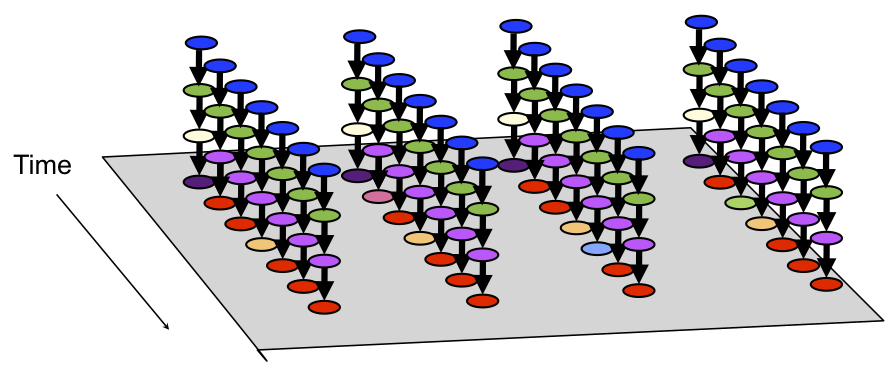
\includegraphics[width=\textwidth]{fig/hpctraceviewer-callpath.png}}
\caption{Logical view of trace call path samples on three dimensions: time, process rank and call path depth.}
\label{fig:hpctraceviewer-callpath}
\end{figure}

\HPCToolkit{}'s \hpctraceviewer{}~\cite{Tallent-MC-etal:2011:ICS-hpctoolkit-scalable-tracing} is a time-centric user interface for interactive examination of a sample-based time series (hereafter referred to as a trace) view of a program execution.
 \hpctraceviewer{} can interactively present a large-scale execution trace without concern for the scale of parallelism it represents.

To collect a trace for a program execution, one must instruct \HPCToolkit{}'s measurement system to collect a trace. 
When launching a dynamically-linked executable with \hpcrun{}, add the {\tt -t } flag to enable tracing. 
When launching a statically-linked executable, set the environment variable \verb|HPCRUN_TRACE=1| to enable tracing. 
When collecting a trace, one must also specify a metric to measure.  The best way to collect a useful trace is to asynchronously sample the execution with a time-based metric such as {\tt REALTIME}, {\tt CYCLES}, or {\tt WALLCLOCK} (Blue Gene/Q only).

As shown in Figure~\ref{fig:hpctraceviewer-callpath},  call path traces consist of data in three dimensions: \emph{process/thread rank}, \emph{time}, and \emph{call path} depth.
A \emph{\crosshair} in \hpctraceviewer{} is defined by a triplet $(p,t,d)$ where $p$ is the selected process/thread rank, $t$ is the selected time, and $d$ is the selected call path depth. 

\hpctraceviewer{}'s  \emph{\traceview} (Section~\ref{sec:traceview}) renders a view of processes and threads over time. \hpctraceviewer{}'s  \emph{\depthview} (Section~\ref{sec:depthview}) shows the call path depth over time for the thread selected by the cursor. \hpctraceviewer{}'s  \emph{\callview}  (Section~\ref{sec:callview}) shows the call path associated with the thread and time pair specified by the cursor. 
Each of these views plays a role for understanding an application's performance.

In \hpctraceviewer, each procedure is assigned specific color. Figure~\ref{fig:hpctraceviewer-callpath} shows that at depth 1   each call path has the same color: blue. This node represents the main program that serves as the root of the call chain in all process at all times. At depth 2, all processes have a green node, which indicates another procedure. 
At depth 3, in the first time step all processes  have a yellow node; in subsequent time steps they have purple nodes.
This might indicate that the processes first are observed in an initialization procedure (represented by yellow) and later observed in a solve procedure (represented by purple). The pattern of colors that appears in a particular depth slice of the \traceview{} enables a user to visually identify inefficiencies such as load imbalance and serialization.

% ===========================================================================
% ===========================================================================

\section{Launching}

Requirements to launch \hpctraceviewer:
\begin{itemize}
 \item On all platforms: Java 8. At the moment \hpcviewer{} cannot run with Java 9 or newer.
 \item On Linux: GTK.
\end{itemize}

\hpctraceviewer{} can either be launched from a command line (Linux platforms) or by clicking the \hpctraceviewer{} icon (for Windows, Mac OS X, and Linux platforms).
The command line syntax is as follows:
\begin{quote}
\begin{verbatim}
  hpctraceviewer [options] [<hpctoolkit-database>]
\end{verbatim}
\end{quote}
Here, \texttt{<hpctoolkit-database>} is an optional argument to load a database automatically.
Without this argument, \hpctraceviewer{} will prompt for the location of a database. Possible options for \hpctraceviewer{}  are shown in the table below:\\

\begin{centering}
\begin{tabular}{|l|p{4.1in}|}\hline\hline
 \verb|-h, --help|   &
 	Print a help message. \\\hline
 \verb|-jh, --java-heap| {\em size}  & 
  	Set the JVM maximum heap size for this execution of \hpctraceviewer{}. The value of {\em size} must be 
	in megabytes (M) or gigabytes (G). For example, one can specify a {\em size}  of 3 gigabytes as either 
	3076M or 3G.\\\hline\hline
 \end{tabular}
 \end{centering}
 \vspace{2ex}

On Linux, when  \hpctraceviewer{}  is installed using its \verb|install| script, the \verb|install| script chooses a default  maximum size for the Java heap on the current platform. When analyzing traces for large and complex applications, it may be necessary to use the \verb|--java-heap| option to specify a larger heap size for  \hpctraceviewer{}.

% ===========================================================================
% ===========================================================================

\section{Views}

\begin{figure}[t]
\centering{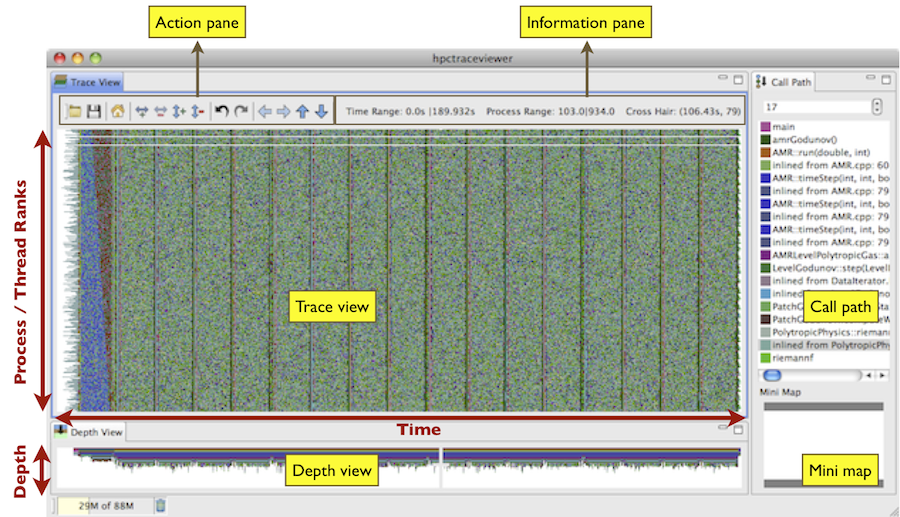
\includegraphics[width=.8\textwidth]{fig/hpctraceviewer-legend.png}}
\caption{A screenshot of \hpctraceviewer{}'s interface.}
\label{fig:hpctraceviewer-legend}
\end{figure}

\begin{figure}[t]
\centering{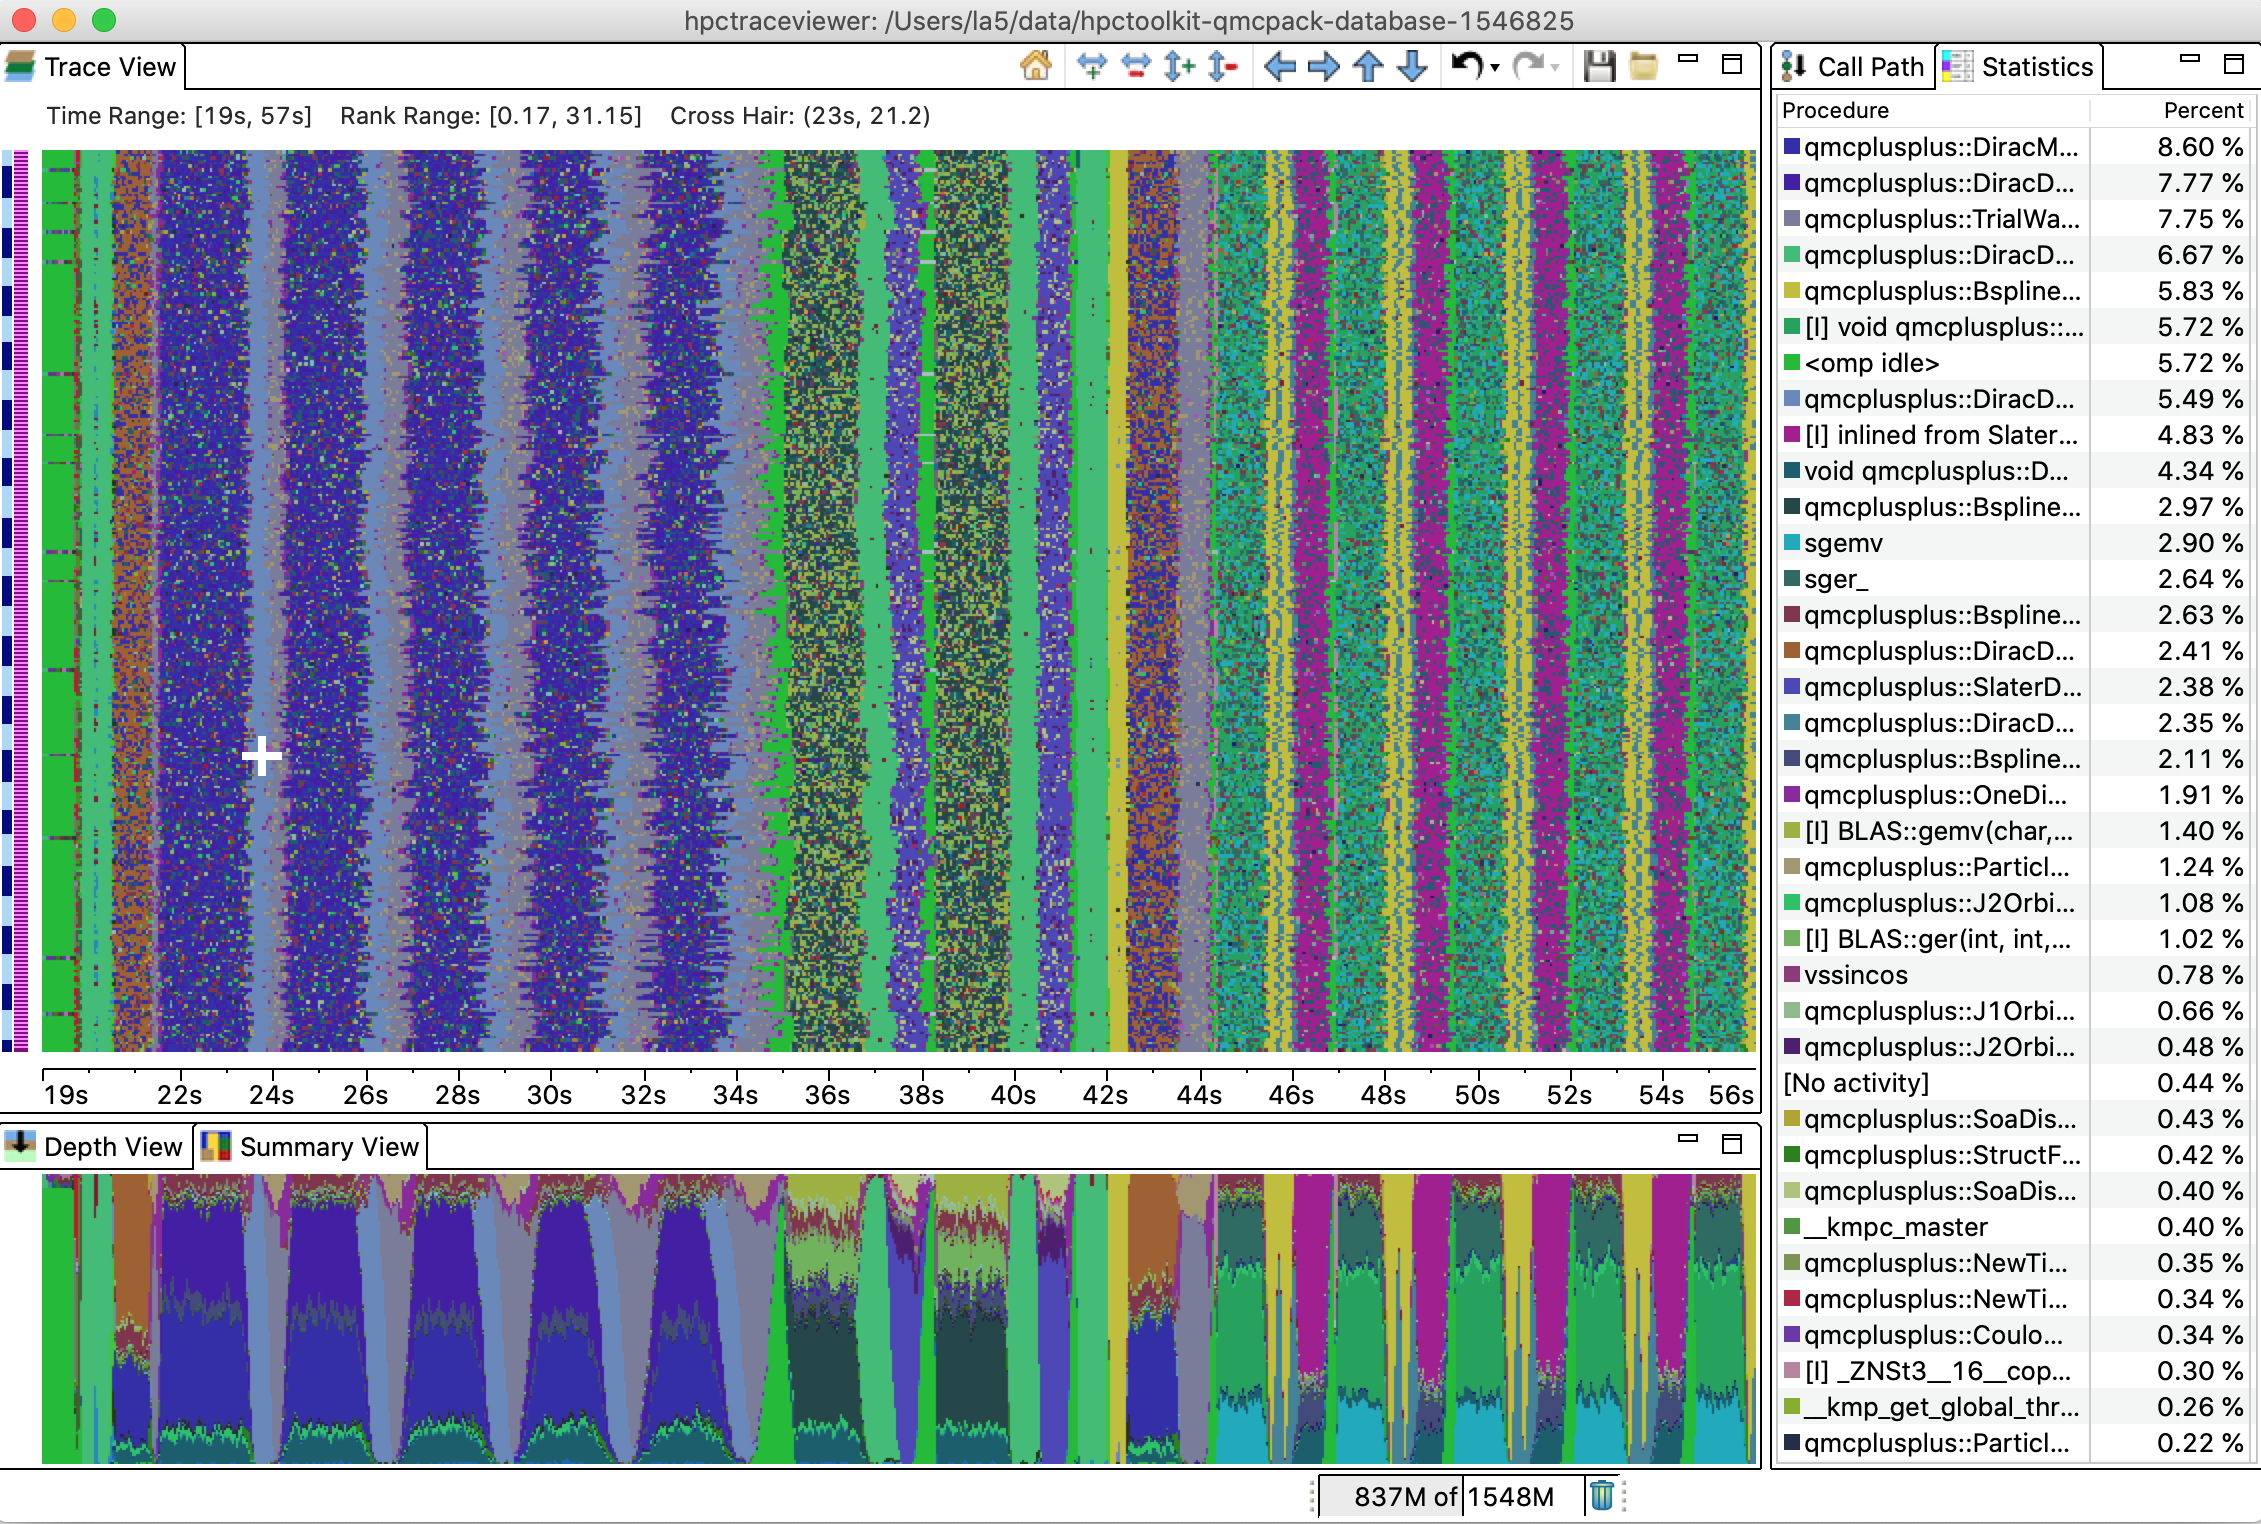
\includegraphics[width=.8\textwidth]{fig/hpctraceviewer-stat.png}}
\caption{A screenshot of \hpctraceviewer{}'s interface showing the \summaryview{} and \statview.}
\label{fig:hpctraceviewer-stat}
\end{figure}

Figures~\ref{fig:hpctraceviewer-legend} and~\ref{fig:hpctraceviewer-stat} show screenshots of \hpctraceviewer{}'s user interface presenting a call path profile.
Figure~\ref{fig:hpctraceviewer-legend} highlights \hpctraceviewer{}'s four principal window panes: \traceview, \depthview, \callview{} and \miniview, 
while Figure\ref{fig:hpctraceviewer-stat} shows additional two window panes: \summaryview{} and \statview.

\begin{itemize}
\item \textbf{\traceview} (top, left pane):
  This is \hpctraceviewer{}'s primary view.
  This view, which is similar to a conventional process/time (or space/time) view, shows time on the horizontal axis and process (or thread) rank on the vertical axis; time moves from left to right.
  Compared to typical process/time views, there is one key difference.
  To show call path hierarchy, the view is actually a user-controllable slice of the process/time/call-path space.
  Given a call path depth, the view shows the color of the currently active procedure at a given time and process rank.
  (If the requested depth is deeper than a particular call path, then \hpctraceviewer{} simply displays the deepest procedure frame and, space permitting, overlays an annotation indicating the fact that this frame represents a shallower depth.)

  \hpctraceviewer{} assigns colors to procedures based on (static) source code procedures.
  Although the color assignment is currently random, it is consistent across the different views.
  Thus, the same color within the Trace and Depth Views refers to the same procedure.

  The Trace View has a white \crosshair{} that represents a selected point in time and process space.
  For this selected point, the Call Path View shows the corresponding call path.
  The Depth View shows the selected process.

\item \textbf{\depthview} (tab in bottom, left pane):
  This is a call-path/time view for the process rank selected by the \traceview's \crosshair{}.
  Given a process rank, the view shows for each virtual time along the horizontal axis a stylized call path along the vertical axis, where `main' is at the top and leaves (samples) are at the bottom.
  In other words, this view shows for the whole time range, in qualitative fashion, what the Call Path View shows for a selected point.
  The horizontal time axis is exactly aligned with the Trace View's time axis; and the colors are consistent across both views.
  This view has its own \crosshair{} that corresponds to the currently selected time and call path depth.

\item \textbf{\summaryview} (tab in bottom, left pane):
  The view shows for the whole time range dislayed, the proportion of each subroutine in a certain time.
  Similar to Depth view, the time range in Summary reflects to the time range in the Trace view. 

\item \textbf{\callview} (tab in top, right pane):
  This view shows two things: (1) the current call path depth that defines the hierarchical slice shown in the Trace View; and (2) the actual call path for the point selected by the Trace View's \crosshair{}.
  (To easily coordinate the call path depth value with the call path, the Call Path View currently suppresses details such as loop structure and call sites; we may use indentation or other techniques to display this in the future.)

\item \textbf{\statview} (tab in top, right pane):
  This view shows the list of procedures active  in the  space-time region shown in the Trace View at the current Call Path Depth. Each procedure's percentage in the \statview{} indicates the percentage of pixels in the Trace View pane that are filled with this procedure's color at the current Call Path Depth. When the Trace View is navigated to show a new time-space interval  or the Call Path Depth is  changed, the statistics view will  update its list of procedures and the percentage of execution time to reflect the new space-time interval or depth selection.
 

\item \textbf{\miniview} (right, bottom):
  The Mini Map shows, relative to the process/time dimensions, the portion of the execution shown by the Trace View.
  The Mini Map enables one to zoom and to move from one close-up to another quickly.

\end{itemize}

% ===========================================================================
% ===========================================================================

\subsection{\traceview}
\label{sec:traceview}

\traceview{} is divided into two parts: the top part which contains \emph{action pane} and the \emph{information pane}, and the main view which displays the traces. 

The buttons in the action pane are the following:
\begin{itemize}

\item \textbf{Home} 
\includegraphics[scale=.5]{fig/hpctraceviewer-button-home-screen.png} : Resetting the view configuration into the original view, i.e., viewing traces for all times and processes.
\item \textbf{Horiontal zoom in 
\includegraphics{fig/hpctraceviewer-button-zoom-in-time.png} / out }
\includegraphics{fig/hpctraceviewer-button-zoom-out-time.png} : Zooming in/out the time dimension of the traces. 
\item \textbf{Vertical zoom in 
\includegraphics[scale=.5]{fig/hpctraceviewer-button-zoom-in-process.png} / out 
\includegraphics[scale=.5]{fig/hpctraceviewer-button-zoom-out-process.png} }: Zooming in/out the process dimension of the traces.
\item \textbf{Navigation buttons} 
\includegraphics[scale=.5]{fig/hpctraceviewer-button-go-east.png}, 
\includegraphics[scale=.5]{fig/hpctraceviewer-button-go-west.png}, 
\includegraphics[scale=.5]{fig/hpctraceviewer-button-go-north.png}, 
\includegraphics[scale=.5]{fig/hpctraceviewer-button-go-south.png} : Navigating the trace view to the left, right, up and bottom, respectively. It is also possible to navigate with the arrow keys in the keyboard. Since \traceview{} does not support scrool bars, the only way to navigate is through navigation buttons (or arrow keys).
\item \textbf{Undo} 
\includegraphics[scale=.5]{fig/hpctraceviewer-button-undo.png} : Canceling the action of zoom or navigation and returning back to the previous view configuration.
\item \textbf{Redo} 
\includegraphics[scale=.5]{fig/hpctraceviewer-button-redo.png} : Redoing of previously undo change of view configuration.
\item \textbf{Save} 
\includegraphics[scale=.5]{fig/hpctraceviewer-button-save.png}  / \textbf{Open 
\includegraphics[scale=.7]{fig/hpctraceviewer-button-open.png} a view configuration} : Saving/loading a saved view configuration. 
A view configuration file contains the information about the process/thread and time ranges shown, the selected depth, and the position of the \crosshair{}. 
It is recommended to store the view configuration file in the same directory as the database to ensure that the view configuration file matches the database since a configuration does not store its associated database. 
Although it is possible to open a view configuration file associated with a different database, it is not recommended since each database has different time/process dimensions and depth.


\end{itemize}

At the top of an execution's \traceview{} pane is some information about the data shown in the pane.
\begin{itemize}
 \item \textbf{Time Range}. The time interval shown along the horizontal dimension. 
 \item \textbf{Process Range}. The range of process/thread ranks shown along the vertical dimension. Ranks are formatted using the following notation:
\begin{verbatim}
  <process_id> . <thread_id>
\end{verbatim}
Hence, if the ranks are 0.0, 0.1, \dots{} 31.0, 31.1 it means that there are 32 MPI processes [0..31], each with two threads [0..1].

 \item \textbf{Cross Hair}. The \crosshair{} indicates the current cursor position in the time and process/thread dimensions. 
\end{itemize}

% ===========================================================================
% ===========================================================================
\subsection{\depthview}
\label{sec:depthview}

\depthview{} shows all the call path for a certain time range $[t_1,t_2]= \{t | t_1\leq t\leq t_2\}$ in a specified process rank $p$. The content of \depthview{} is always consistent with the position of the \crosshair{} in \traceview{}.
For instance once the user clicks in process $p$ and time $t$, while the current depth of call path is $d$, then the \depthview's content is updated to display all the call path of process $p$ and shows its \crosshair{} on the time $t$ and the call path depth $d$.

On the other hand, any user action such as \crosshair{} and time range selection in \depthview{} will update the content within \traceview. Similarly, the selection of new call path depth in \callview{} invokes a new position in \depthview.

In \depthview{} a user can specify a new \crosshair{} time and a new time range.
\paragraph{Specifying a new \crosshair{} time.} Selecting a new \crosshair{} time $t$ can be performed by clicking a pixel within \depthview{}. This will update the \crosshair{} in \traceview{} and the call path in \callview.

\paragraph{Selecting a new time range.} Selecting a new time range $[t_m,t_n]= \{t | t_m\leq t\leq t_n\}$ is performed by first clicking the position of $t_m$ and drag the cursor to the position of $t_n$. A new content in \depthview{} and \traceview{} is then updated. Note that this action will not update the call path in \callview{} since it does not change the position of the \crosshair.


% ===========================================================================
% ===========================================================================
\subsection{\summaryview}
\label{sec:summaryview}

\summaryview{} presents the proportion of number of calls of time $t$ across the current displayed rank of proces $p$. 
Similar to \depthview, the time range in \summaryview{} is always consistent with the time range in \traceview{}.


% ===========================================================================
% ===========================================================================
\subsection{\callview}
\label{sec:callview}

\begin{figure}[t]
\centering{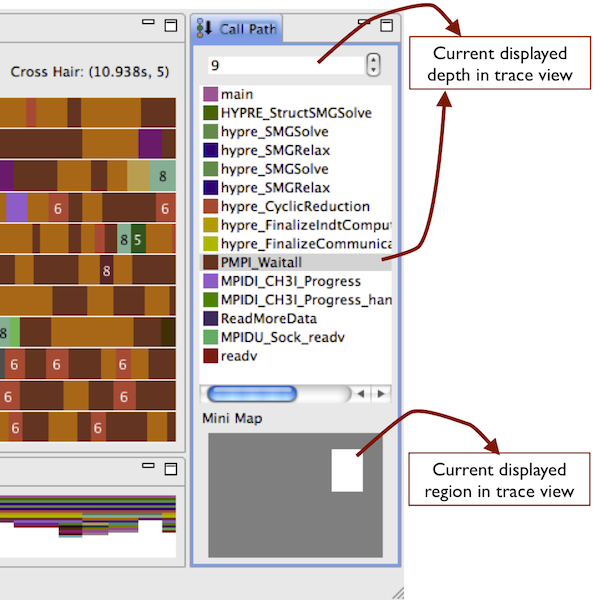
\includegraphics{fig/hpctraceviewer-callpath-legend.png}}
\caption{An annotated screenshot of \hpctraceviewer{}'s \callview.}
\label{fig:hpctraceviewer-callpath-legend}
\end{figure}

This view lists the call path of process $p$ and time $t$ specified in \traceview{} and \depthview.
Figure~\ref{fig:hpctraceviewer-callpath-legend} shows a call path from depth $0$ to depth $14$, and the current depth is $9$ as shown in the depth editor (located on the top part of the view).

In this view, the user can select the depth dimension of \traceview{} by either typing the depth in the depth editor or selecting a procedure in the table of call path.

% ===========================================================================
% ===========================================================================
\subsection{\miniview}
\label{sec:miniview}

The \miniview{} shows, relative to the process/time dimensions, the portion of the execution shown by the \traceview.
In \miniview{}, the user can select a new process/time $(p_a,t_a),(p_b,t_b)$ dimensions by clicking the first process/time position $(p_a,t_a)$ and then drag the cursor to the second position $(p_b,t_b)$.
The user can also moving the current selected region to another region by clicking the white rectangle and drag it to the new place.


% ===========================================================================
% ===========================================================================

\begin{figure}[t]
\centering{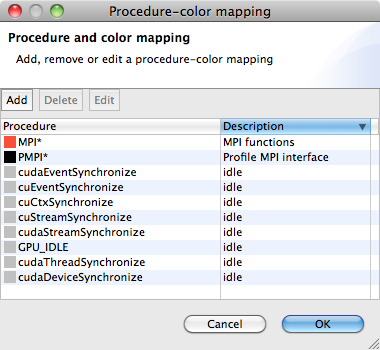
\includegraphics[width=3.4in]{fig/hpctraceviewer-dialog-mapping}}
\caption{Procedure-color mapping dialog box. This window shows that any procedure names that match with "MPI*" pattern are assigned with red, while procedures that match with "PMPI*" pattern are assigned with color black.}
\label{fig:hpctraceviewer-mapping}
\end{figure}

\begin{figure}[t]
\centering{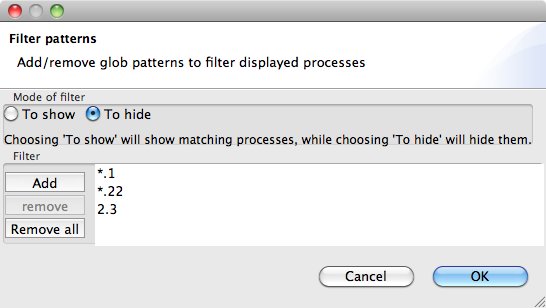
\includegraphics[width=4in]{fig/hpctraceviewer-dialog-filter.png}}
\caption{Rank filter dialog box. This window shows that all rank IDs that match with the list of patterns will be hidden from the display. For example, ranks 1.1, 2.1, 1.22, 1.3 will be hidden.}
\label{fig:hpctraceviewer-filter}
\end{figure}


\section{Menus}
\hpctraceviewer{} provides three main menus:
\begin{itemize}
 \item \textbf{File} menu which contains two sub menus:
 \begin{itemize}
   \item \textbf{Open database}: to load a database experiment directory. The directory has to contain \texttt{experiment.xml} (CCT and metric information) or \texttt{callpath.xml} (uniquely CCT information), and \texttt{*.hpctrace} or \texttt{experiment.mt} files which provide trace information.
   \item \textbf{Exit}: to quit the application.
 \end{itemize}
 \item \textbf{View} menu to enhance appearance which contains two sub menus:
 \begin{itemize}
   \item \textbf{Show debug info}: to enable/disable the display of debugging information in the form of `$a(b)$' where $a$ is the maximum depth (this number is shown if the current depth reaches the maximum depth) and $b$ is the number of records on the trace view. 
The number of records can be useful to identify blocking procedures (such as I/O operations). Note: the numbers are displayed only if there's enough space in the process time line.
   \item \textbf{Using midpoint painting}: if checked, the trace painting will use \emph{midpoint} painting algorithm. By using the later, for every samples $S_1$ at time $T_1$, $S_2$ at time $T_2$ and $S_3$ at time $T_3$, \hpctraceviewer{} renders a block from $T_1$ to $\frac{T1+T2}{2}$ to sample $S_1$, and a block from from  $\frac{T1+T2}{2}$ to  $\frac{T2+T3}{2}$ for sample $S_2$, and so forth. 
If the menu is not checked, then a simpler \emph{rightmost} algorithm is used: it will render a block from  $T_1$ to $T_2$ for sample $S_1$, and a block from $T_2$ to  $T3$ for sample $S_2$, and so forth.
   \item \textbf{Show procedure-color mapping}: to open a window which shows customized mapping between a procedure pattern and a color (Figure~\ref{fig:hpctraceviewer-mapping}). \hpctraceviewer{} allows users to customize assignment of a pattern of procedure names with a specific color.
   \item \textbf{Filter ranks}: to open a window for selecting which ranks and/or threads should be displayed or hidden (Figure~\ref{fig:hpctraceviewer-filter}). 
Recall that a rank can be a process (e.g. MPI applications), a thread (OpenMP applications) or a process/thread pair (hybrid MPI and OpenMP applications). 
\hpctraceviewer{} allows two types of filtering: either you specify which ranks \textit{to show} or \textit{to hide} (default is to hide). 
To add a pattern to filter, you need to click the "Add" button and type the pattern in the format \texttt{minimum:maximum:stride}. \\
For instance, \texttt{3:7:2} in the process box with the thread box empty will match all threads of processes 3, 5, and 7.\\
To remove a pattern, you have to select the pattern to remove, and click the "Remove" button. Finally, clicking to "Remove all" button will clear the list of patterns.
 \end{itemize}
 \item \textbf{Window} menu to manage the layout of the application. The menu only provide one sub menu:
 \begin{itemize}
  \item \textbf{Reset layout}: to reset the layout to the original one.
 \end{itemize}
\end{itemize}

\hpctraceviewer{} also provides a context menu to save the current image of the view. 
This context menu is available is three views: trace view, depth view and summary view.

% ===========================================================================
% ===========================================================================

\section{GPU Threads}

\hpctraceviewer{} displays activity over time in GPU streams as well as CPU threads. Presently, GPU streams and CPU threads are indexed within a process or MPI rank using a single integer coordinate. To distinguish between GPU threads and CPU threads in this prototype, CPU thread numbers begin at 0 and GPU stream numbers begin at 500. 

Unlike CPU threads, which are sampled, each GPU activity (e.g., a kernel execution or a memory copy)  on a GPU stream or queue is traced. To avoid giving a misleading view of GPU activity on a stream or queue, intervals between GPU activities where the GPU is idle are marked with the placeholder \verb|<no activity>|.

\section{Limitations}

Some important \hpctraceviewer{} limitations are listed below:
\begin{itemize}

\item \textbf{Rendering very long traces may be slow.} \hpctraceviewer{} locates each entry to render along a process/thread timeline using binary search. Thus, for a timeline of length $t$, rendering $n$ samples takes time $n \log t$. 

\item \textbf{Slow rendering of large traces on IBM Power7 and BGQ platforms}.
	Displaying a  trace larger than 2 GB on IBM Power7 and BGQ is very slow. 


\end{itemize}
